% you don't need a template
% use the following one

\documentclass{report}

\usepackage{graphicx}
\graphicspath{{img/}}
\usepackage[a4paper, top=2cm, bottom=2cm, left=3cm, right=3cm]{geometry}


\usepackage{listings}
\lstset{language=Python, basicstyle=\ttfamily\small, frame=single, breaklines=true}

\title{A Labwork 5 Report}
\author{Luc Lacotte}
\date{}

\begin{document}

\maketitle

\section{Introduction}
This labwork is about implementing a Gaussian blur filter and experimenting with shared memory.

\section{Gaussian blur using CPU}
First I implemented the Gaussian blur filter on the CPU.
Here is the function:

\begin{lstlisting}
def gaussian_blur_cpu(image):
    h, w, chan = image.shape
    output_image = np.zeros_like(image)
    image = image.astype(np.int32)

    for y in range(h):
        for x in range(w):
            for c in range(chan):
                out_of_range_pixel_value = 0
                pixel_value = 0
                for ky in range(-3, 4):
                    for kx in range(-3, 4):
                        ly = y + ky
                        lx = x + kx
                        if ly < 0 or ly >= h or lx < 0 or lx >= w:
                            out_of_range_pixel_value += GAUSSIAN_BLUR_MATRIX[ky + 3][kx + 3]
                        else:
                            pixel_value += image[ly, lx, c] * GAUSSIAN_BLUR_MATRIX[ky + 3][kx + 3]
                output_image[y, x, c] = pixel_value // (GAUSSIAN_BLUR_MATRIX_SUM - out_of_range_pixel_value)

    return output_image
\end{lstlisting}

This function is very slow on CPU, I first tried with big images and it took too much time that I stopped the process.
For an image of 597x389, it took more than 6 seconds.

\section{Gaussian blur using GPU}
This time for GPU implementations, I used an image of 108M pixels (12000x9000).

Then I implemented the same function but using, of course, the GPU.
The kernel function is the same as the CPU function, but it uses the thread index to compute the pixel coordinates:

\begin{lstlisting}
@cuda.jit
def gaussian_blur_gpu(src, dst, matrix, matrix_sum):
    tidx = cuda.threadIdx.x + cuda.blockIdx.x * cuda.blockDim.x
    tidy = cuda.threadIdx.y + cuda.blockIdx.y * cuda.blockDim.y
    h, w, chan = src.shape
    if tidx >= w or tidy >= h:
        return
    for c in range(chan):
        out_of_range_pixel_value = 0
        pixel_value = 0
        for ky in range(-3, 4):
            for kx in range(-3, 4):
                ly = tidy + ky
                lx = tidx + kx
                if ly < 0 or ly >= h or lx < 0 or lx >= w:
                    out_of_range_pixel_value += matrix[ky + 3, kx + 3]
                else:
                    pixel_value += src[ly, lx, c] * matrix[ky + 3, kx + 3]
        dst[tidy, tidx, c] = pixel_value // (matrix_sum - out_of_range_pixel_value)
\end{lstlisting}

\section{Using shared memory}
For using shared memory, I couldn't find how I was supposed to implement it, so Gen AI helped me a bit.

\begin{lstlisting}
@cuda.jit
def gaussian_blur_gpu_shared_memory(src, dst, matrix, matrix_sum):
    tile = cuda.shared.array(shape=(32, 32, 3), dtype=numba.uint8)
    tx = cuda.threadIdx.x
    ty = cuda.threadIdx.y
    bx = cuda.blockIdx.x
    by = cuda.blockIdx.y
    bdx = cuda.blockDim.x
    bdy = cuda.blockDim.y
    x = bx * bdx + tx
    y = by * bdy + ty
    h, w, chan = src.shape
    if x >= w or y >= h:
        return
    for c in range(chan):
        tile[ty, tx, c] = src[y, x, c]
    cuda.syncthreads()
    for c in range(chan):
        out_of_range_pixel_value = 0
        pixel_value = 0
        for ky in range(-3, 4):
            for kx in range(-3, 4):
                ly = ty + ky
                lx = tx + kx
                if ly < 0 or ly >= bdy or lx < 0 or lx >= bdx or y + ky >= h or x + kx >= w:
                    out_of_range_pixel_value += matrix[ky + 3, kx + 3]
                else:
                    pixel_value += tile[ly, lx, c] * matrix[ky + 3, kx + 3]
        dst[y, x, c] = pixel_value // (matrix_sum - out_of_range_pixel_value)
\end{lstlisting}

\section{Compare with and without shared memory}

\begin{figure}[h]
\centering
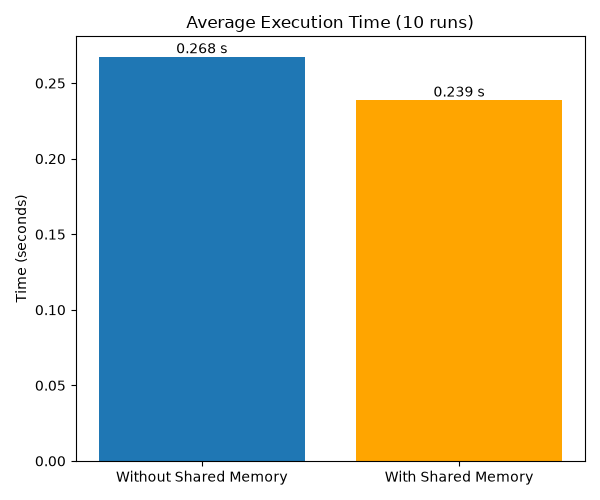
\includegraphics[width=0.6\textwidth]{execution_times.png}
\caption{Execution times of the Gaussian blur filter on global memory and shared memory.}
\end{figure}

We can see that over some iterations, shared memory is a bit faster.

\section{Experimenting with block size}

To experiment with block size, I tried automating it in the script with some loops, but because the shared array size needs to be known at compile time, I created a factory.

\begin{lstlisting}
def gaussian_blur_gpu_shared_memory_factory(blockSizeX, blockSizeY):
    @cuda.jit
    def gaussian_blur_gpu_shared_memory_variable(src, dst, matrix, matrix_sum):
        tile = cuda.shared.array(shape=(blockSizeY, blockSizeX, 3), dtype=numba.uint8)
        tx = cuda.threadIdx.x
        ty = cuda.threadIdx.y
        bx = cuda.blockIdx.x
        by = cuda.blockIdx.y
        bdx = cuda.blockDim.x
        bdy = cuda.blockDim.y
        x = bx * bdx + tx
        y = by * bdy + ty
        h, w, chan = src.shape
        if x >= w or y >= h:
            return
        for c in range(chan):
            tile[ty, tx, c] = src[y, x, c]
        cuda.syncthreads()
        for c in range(chan):
            out_of_range_pixel_value = 0
            pixel_value = 0
            for ky in range(-3, 4):
                for kx in range(-3, 4):
                    ly = ty + ky
                    lx = tx + kx
                    if ly < 0 or ly >= bdy or lx < 0 or lx >= bdx or y + ky >= h or x + kx >= w:
                        out_of_range_pixel_value += matrix[ky + 3, kx + 3]
                    else:
                        pixel_value += tile[ly, lx, c] * matrix[ky + 3, kx + 3]
            dst[y, x, c] = pixel_value // (matrix_sum - out_of_range_pixel_value)

    return gaussian_blur_gpu_shared_memory_variable
\end{lstlisting}

With this, I have a function that returns the kernel function with the block size I want.

Here are the results:

\begin{figure}[h]
\centering
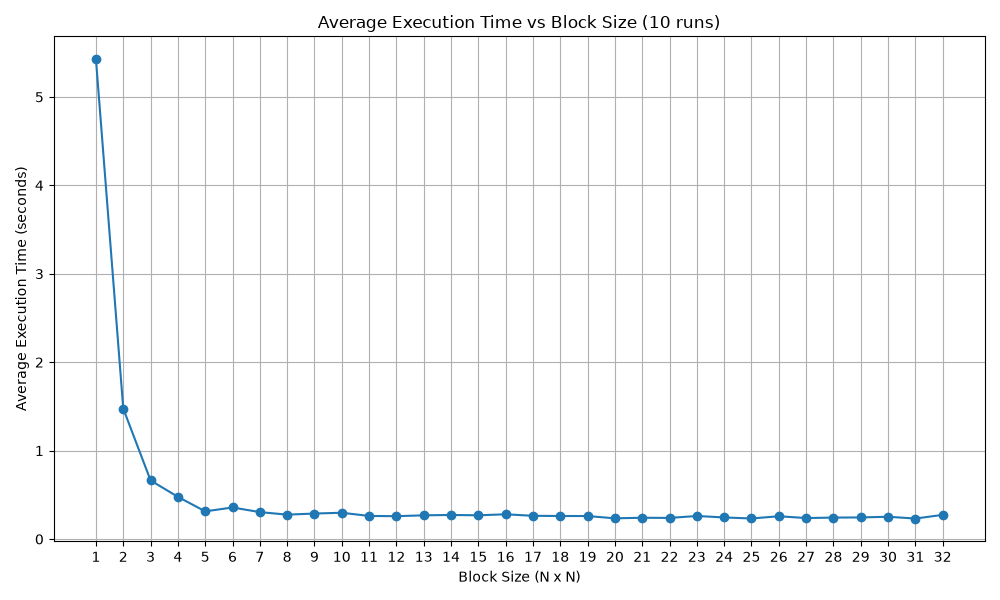
\includegraphics[width=0.7\textwidth]{execution_times_block_size.png}
\caption{Execution times of the Gaussian blur filter on shared memory with different block sizes.}
\end{figure}

We can see that very small block sizes are very slow, but once we reach a block size of 8x8, the execution time remains approximately the same until the maximum block size of 32x32.

\end{document}